
\chapter{Architecture}
%Her beskrives den overordnede systemarkitektur vha. en domænemodel efterfulgt af SysML/UML. Der tages stilling til hvilke dele af projektet, der skal realiseres i HW og hvilke der skal realiseres vha. SW. De vigtigste dele af arkitekturen beskrives for systemets HW og SW i en sådan grad, at læseren får det fornødne overblik over systemet. Der fokuseres på opdeling i blokke, moduler, pakker, klasser etc. Der fokuseres ligeledes på hvordan disse blokke/moduler/pakker/klasser kommunikerer indbyrdes, dvs. de overordnede signaler/protokoller beskrives. For beskrivelse af detaljer angives reference til jeres ”arkitekturdokument” i projektets bilag.

In this section the hardware and software architecture of the system will be discussed. The architecture is the ground work that enables the team to go ahead with designing the system. This essentially boils down to taking the requirements and dividing it in to blocks, modules, etc.

For a more in depth explanation of the different subjects discussed in this section, refer to the \nameref{sec:sys-architecture}, section~\ref{sec:sys-architecture}, on page~\pageref{sec:sys-architecture} in the documentation.

\section{Hardware architecture}
To get a better understanding of the components which are needed for this system, a block definition diagram or BDD was devised, as seen in figure~\ref{fig:generalbdd}. 

\begin{figure}[H]
\centering
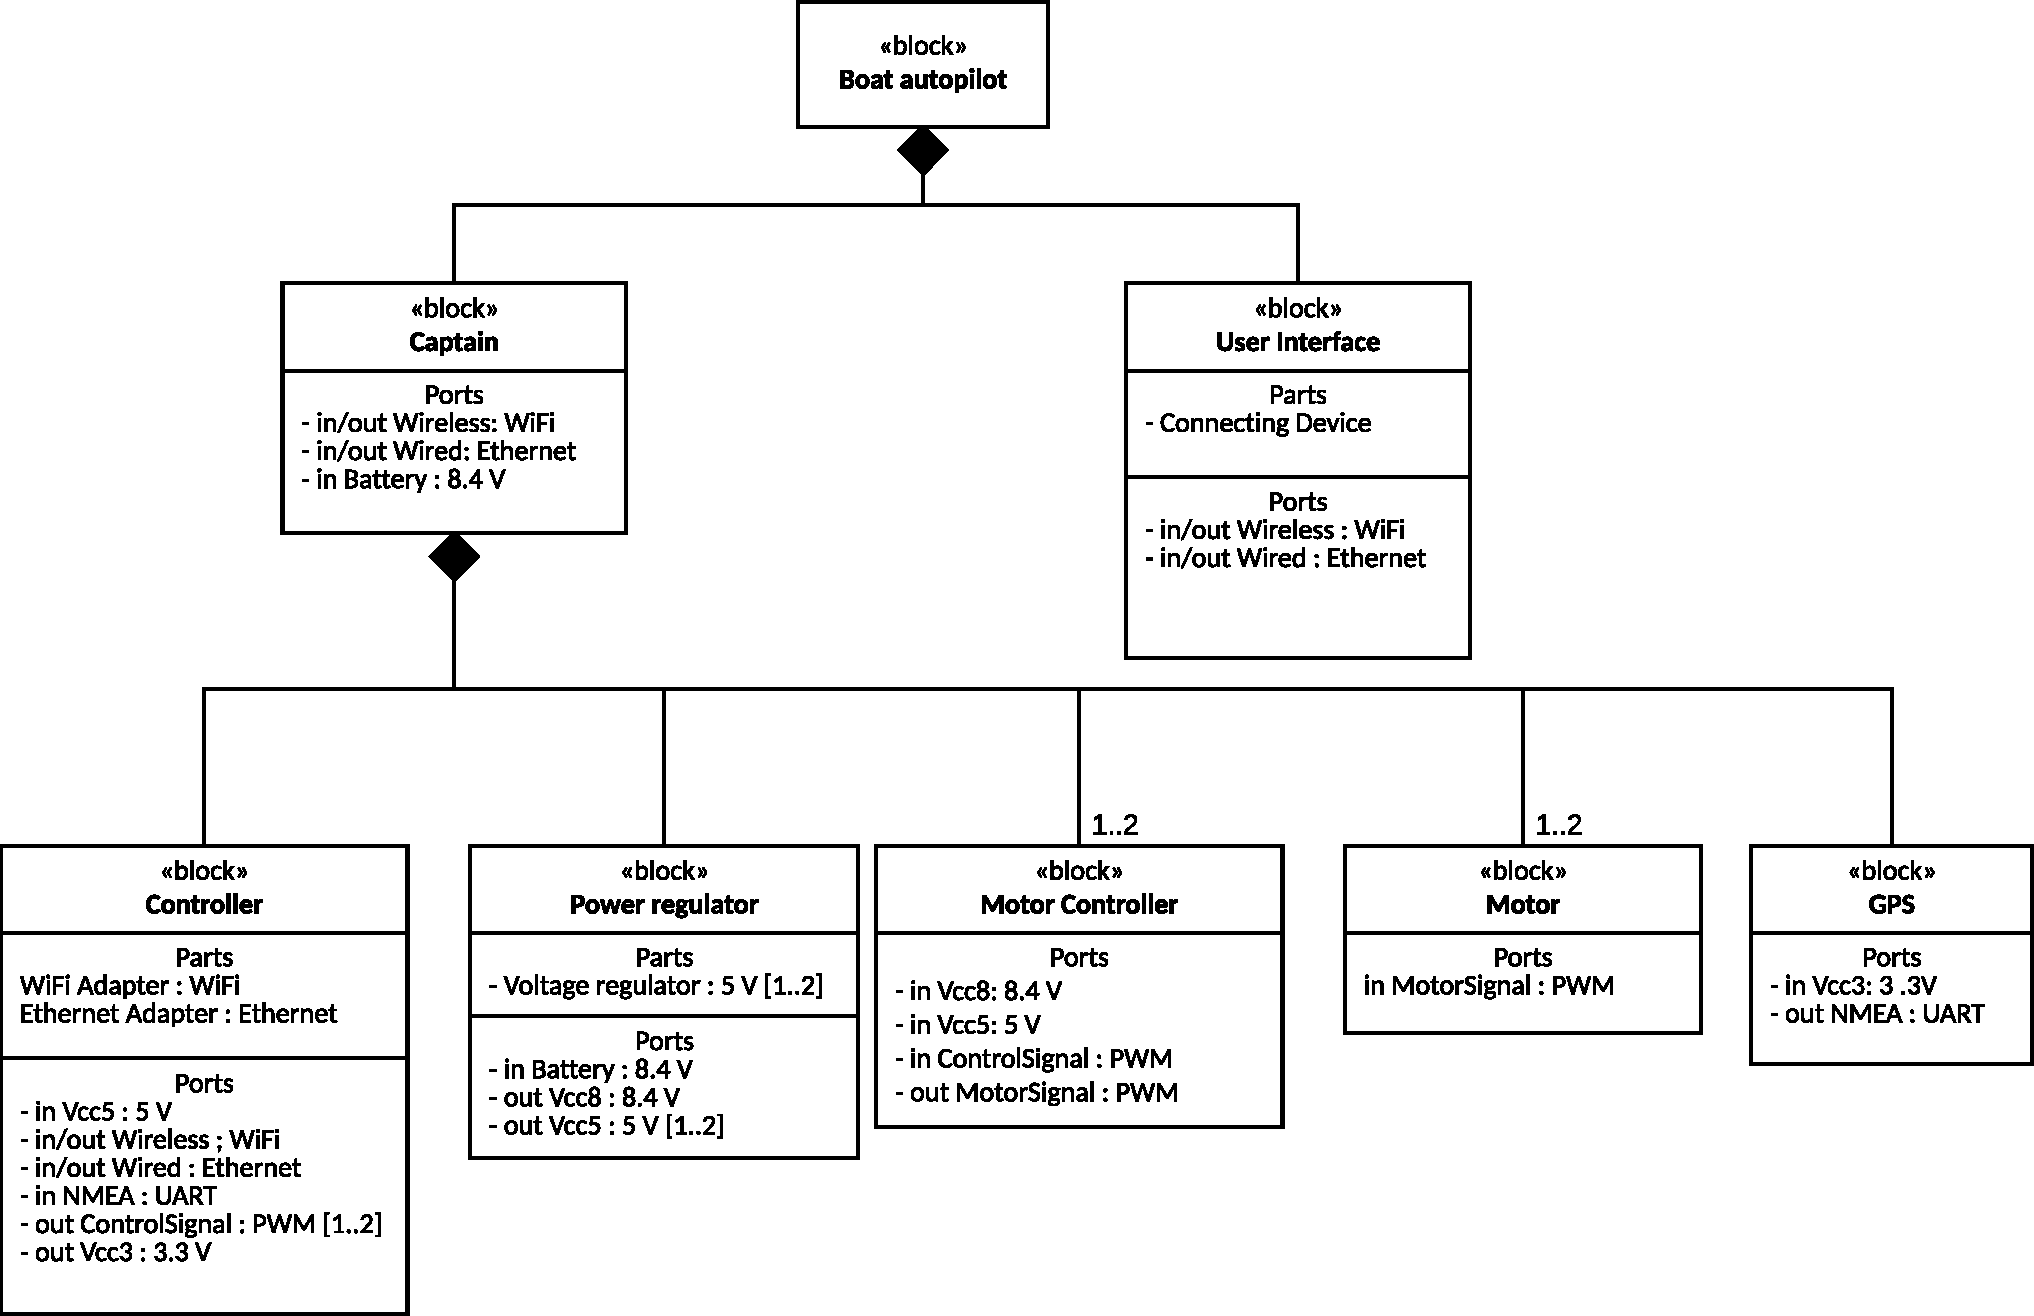
\includegraphics[width=1\linewidth]{../Appendix/Project/Dokumentation/Images/System_architecture/General_BDD}
\caption{General block definition diagram (BDD)}
\label{fig:generalbdd}
\end{figure}

The Boat autopilot can be broken down into two separate parts. One is the user interface; this is a client's personal computer. This personal computer needs to have WiFi and an Ethernet port, this is so it can connect to the system. The system is the other part, and it has been named Captain. 

In this diagram, Captain is the hardware platform for this project, and it also requires WiFi and an Ethernet port, so it can be connected to the user interface. Furthermore it needs an external battery to power it.  Captain is also built up of subcomponents, or parts; a GPS receiver, 1 or 2 motors, 1 or 2 motor controllers, a power regulator, and a controller unit. The controller can be considered the brains of the operation; it communicates with the user interface, dictates what the motors should do, and it reads from the GPS receiver. The power regulator is used to regulate the battery voltage, so the controller, the motor, and the motor controller can all use it simultaneously. The motor controller drives the motor according to the control signals from the controller. 

With these blocks now defined, an IBD or internal block diagram can be created, seen in figure~\ref{fig:generalibd}. This diagram describes how the different blocks of the BDD connect to each other, via the signals that are defined in the BDD as well. A full signal list and description can be found in the documentation in section~\ref{sec:general_ibd} on page~\pageref{sec:general_ibd}.
\begin{figure}[H]
\centering
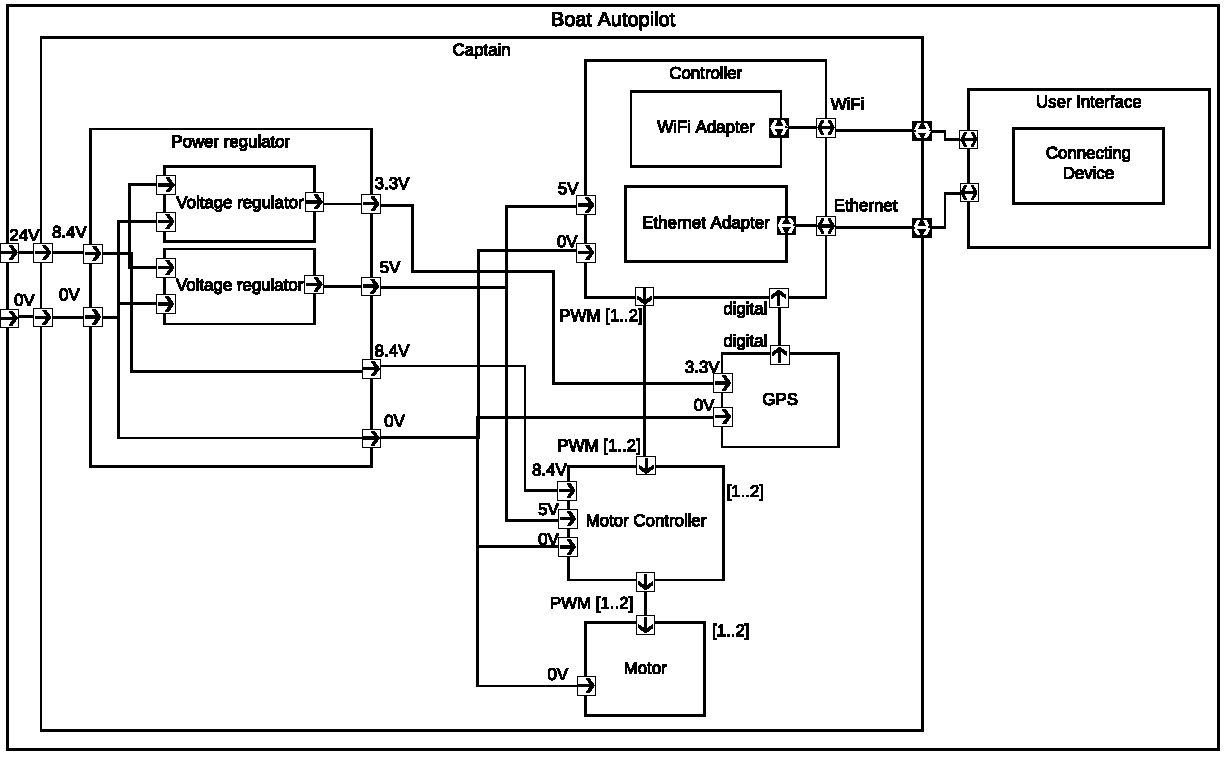
\includegraphics[width=1\linewidth]{../Appendix/Project/Dokumentation/Images/System_architecture/General_IBD}
\caption{General internal block diagram (IBD)}
\label{fig:generalibd}
\end{figure}

\section{Software architecture}
The software architecture is described with a domain model, an application model and several sequence diagrams. 

We start out by having a look at the domain model, seen in figure~\ref{fig:domainmodel}. The domain model is used to describe how the system should behave when an actor interacts with it. The domain model shows how the user or technician can interact with the web interface, and how it then communicates with the controller. The controller controls the motors, which in turn change the boat's position. This then affects what the GPS receiver reads, and this information is then passed on to the controller. This loop continues until the boat has reached its destination.

\begin{figure}[H]
\centering
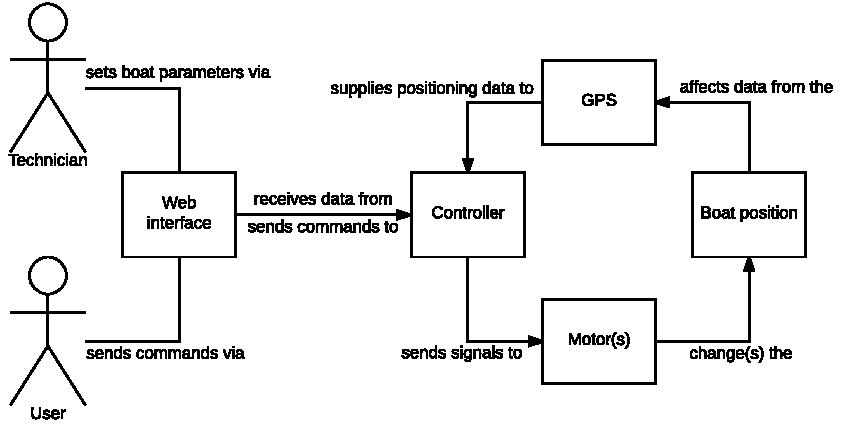
\includegraphics[width=1\linewidth]{../Appendix/Project/Dokumentation/Images/System_architecture/Domain_Model}
\caption{Domain model}
\label{fig:domainmodel}
\end{figure}

With a domain model and use cases already defined, an application model can be created for the system, as seen in figure~\ref{fig:applicationmodel}. This diagram describes the functionality of the block from the domain model, and also classifies the blocks as being either a boundary, control or an entity. A boundary block is something that interacts with the real world, a control block is the block that mediates functionality of boundary blocks and entity blocks. The entity block is a representation of information.

\begin{figure}[H]
\centering
\includegraphics[width=1\linewidth]{../Appendix/Project/Dokumentation/Images/System_architecture/Application_Model}
\caption{Application model}
\label{fig:applicationmodel}
\end{figure}

With the functionality of the blocks in place, it is now time to look at the sequence diagrams. There are a number of sequence diagrams, so only a few interesting ones will be discussed in this report. For all the sequence diagrams, have a look in the documentation in section~\ref{sec:soft-architecture} on page~\pageref{sec:soft-architecture}.

The sequence diagrams follow the use cases, so to start off, the ones corresponding to use cases discussed in the requirements section will be looked at. These are; use case 3 - "Edit parameter profile", use case 11 - "Calculate coverage path", use case 12 - "Run coverage path", and use case 5 - "Request diagnostics". 

Figure~\ref{fig:usecase3sd} explains how a technician edits a parameter. First the parameter profile is displayed, then it is edited by the technician.  

\begin{figure}[H]
\centering
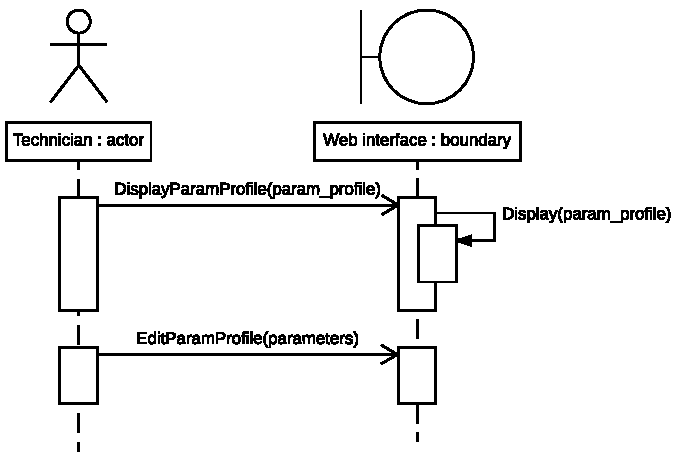
\includegraphics[width=1\linewidth]{../Appendix/Project/Dokumentation/Images/System_architecture/Use_case_3_SD}
\caption{Sequence diagram for use case 3 - "Edit parameter profile"}
\label{fig:usecase3sd}
\end{figure}

Figure~\ref{fig:usecase11sd} is showing how a user commands the system to calculate a coverage path. This is done through the user interface, which tells the controller to calculate a path. The controller uses GPS data to calculate the path and then returns the path to the web interface. The path is then displayed.

\begin{figure}[H]
\centering
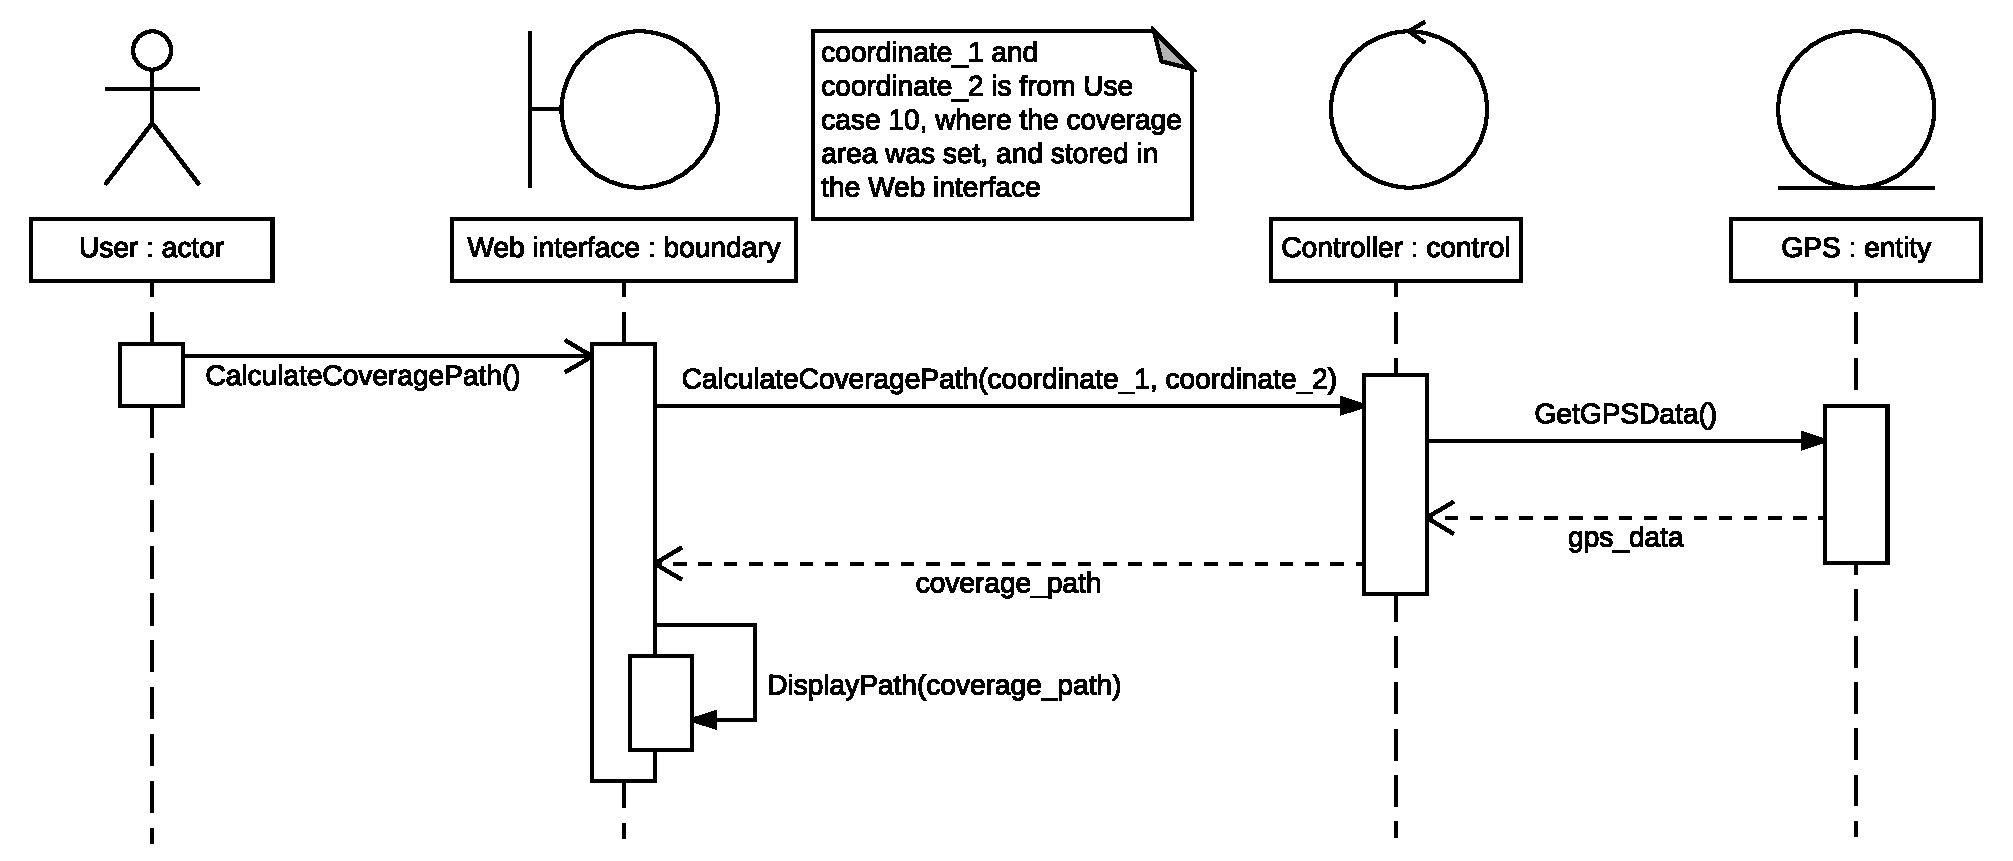
\includegraphics[width=1\linewidth]{../Appendix/Project/Dokumentation/Images/System_architecture/Use_case_11_SD}
\caption{Sequence diagram for use case 11 - "Calculate coverage path"}
\label{fig:usecase11sd}
\end{figure}

Figure~\ref{fig:usecase12sd} illustrates what happens in use case 12. When the user commands the web interface to Run, it relays the message to the controller which in turn starts a loop. This loop gets GPS data and tells the motors how to behave. It then sends the web interface information, enabling the interface to display the boat's position. The controller also calculate the estimated time en-route and the web interface will display it.

\begin{figure}[H]
\centering
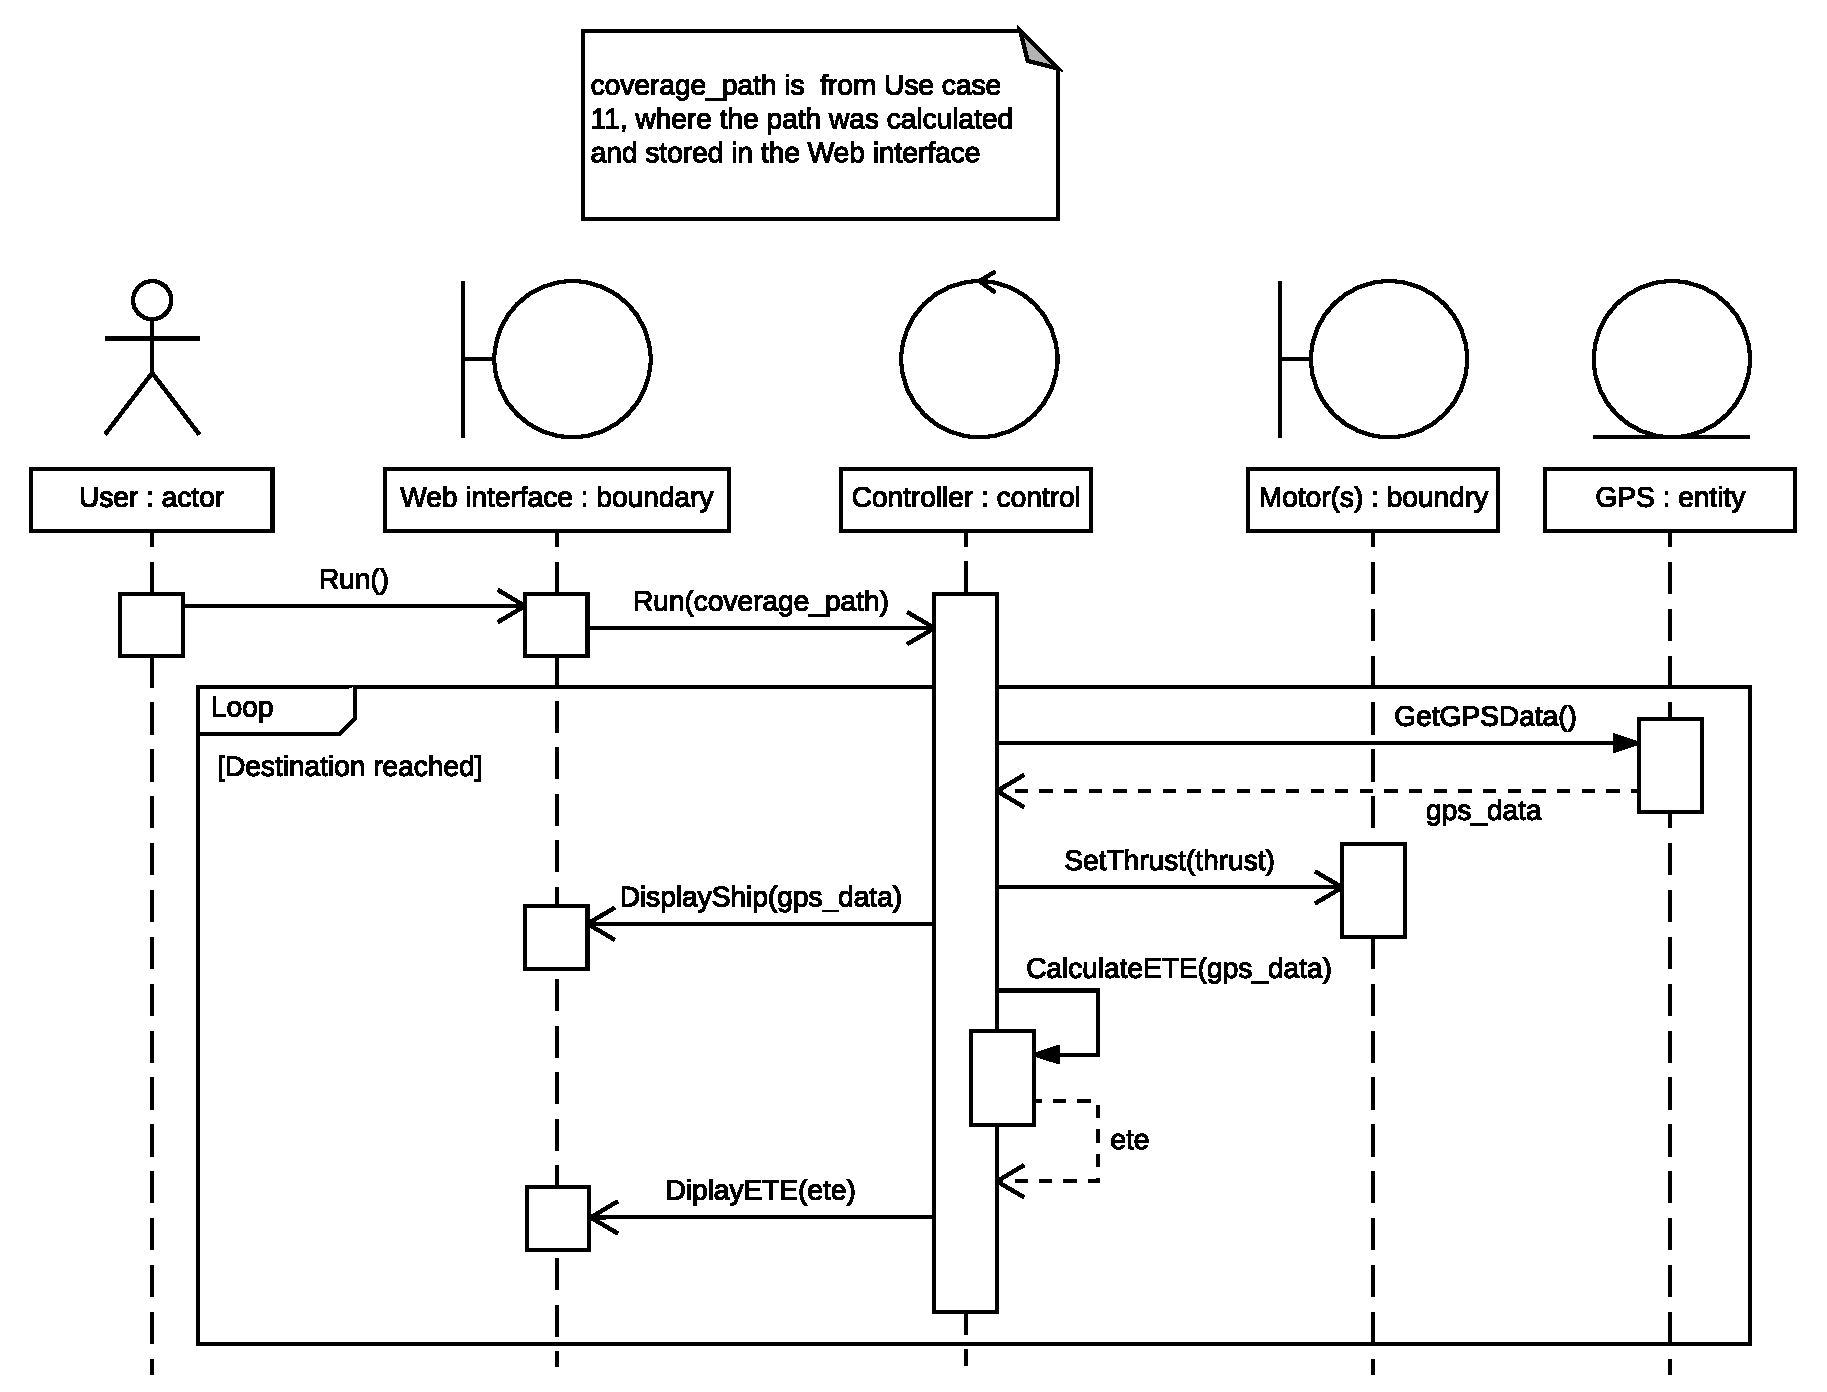
\includegraphics[width=1\linewidth]{../Appendix/Project/Dokumentation/Images/System_architecture/Use_case_12_SD}
\caption{Sequence digram for use case 12 - "Run coverage path"}
\label{fig:usecase12sd}
\end{figure}

Lastly, figure~\ref{fig:usecase5sd} demonstrates how the system acquires and displays diagnostics data. When the user requests diagnostics data, the web interface asks the controller to calculate it. The controller responds by getting the current thrust of the motors and the GPS data along with the GPS diagnostics data. The controller also fetches connection diagnostics from the web interface, all of this is then displayed in the web interface.

\begin{figure}[H]
\centering
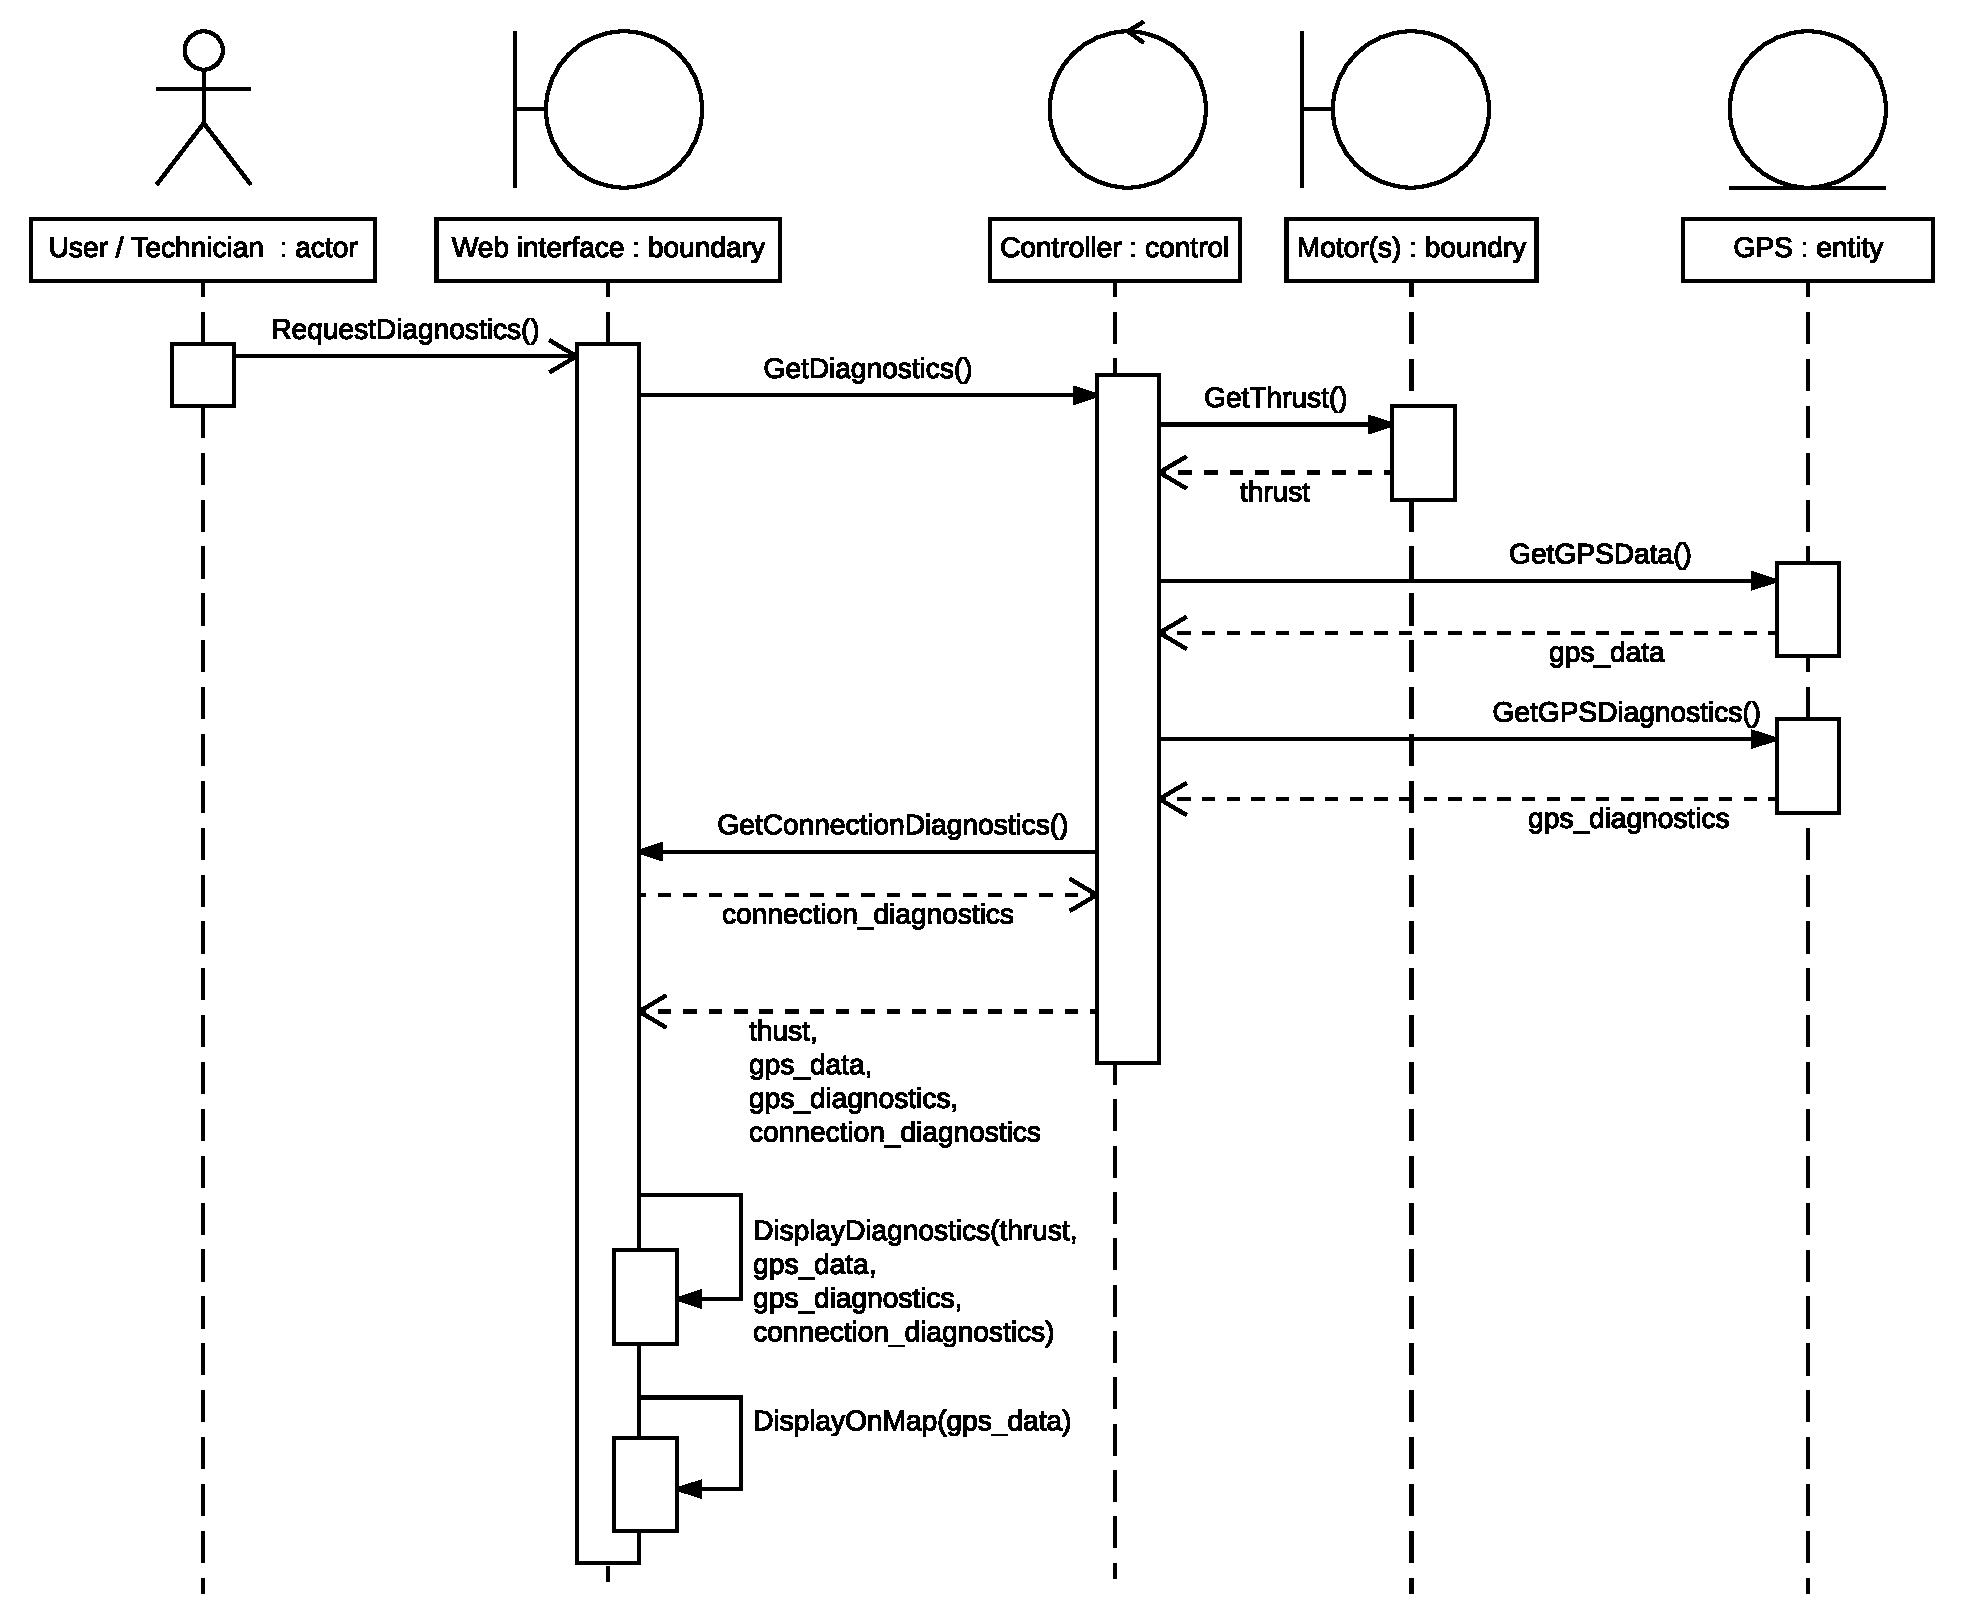
\includegraphics[width=1\linewidth]{../Appendix/Project/Dokumentation/Images/System_architecture/Use_case_5_SD}
\caption{Sequence diagram for use case 5 - "Request diagnostics"}
\label{fig:usecase5sd}
\end{figure}











